%------------------------
% CV in Latex
% Author : Sourabh Bajaj
% Modified by : Abhishek Ramanathapura Satyanarayana
% License : MIT
%------------------------

\documentclass[letterpaper,12pt]{article}

\usepackage{latexsym}
\usepackage[empty]{fullpage}
\usepackage{titlesec}
\usepackage{marvosym}
\usepackage[usenames,dvipsnames]{color}
\usepackage{verbatim}
\usepackage{enumitem}
\usepackage[pdftex]{hyperref}
\usepackage{fancyhdr}
\usepackage{ragged2e}
\usepackage{comment}
\usepackage{graphicx,wrapfig}
\usepackage{fontawesome}
\graphicspath{{./images/}}

\pagestyle{plain}
\fancyhf{} % clear all header and footer fields
\fancyfoot{}
\cfoot{\thepage}
\renewcommand{\headrulewidth}{0pt}
\renewcommand{\footrulewidth}{0pt}

% Adjust margins
% \addtolength{\oddsidemargin}{-0.375in}
% \addtolength{\evensidemargin}{-0.375in}
% \addtolength{\textwidth}{1in}
% \addtolength{\topmargin}{-.5in}
% \addtolength{\textheight}{1.0in}
\usepackage[margin=0.6in]{geometry}

\urlstyle{same}
\raggedbottom
\raggedright
\setlength{\tabcolsep}{0in}

% Sections formatting
\titleformat{\section}{
    \vspace{-4pt}\scshape\raggedright\large
}{}{0em}{}[\color{black}\titlerule \vspace{-5pt}]

%-------------------------
% Custom commands
\newcommand{\resumeItem}[2]{
    \item\small{
        \textbf{#1}{: #2 \vspace{-2pt}}
    }
}

\newcommand{\resumeSubheading}[4]{
    \vspace{-1pt}\item
    \begin{tabular*}{0.97\textwidth}{l@{\extracolsep{\fill}}r}
        \textbf{#1} & #2 \\
        \textit{\small#3} & \textit{\small #4} \\
    \end{tabular*}\vspace{-5pt}
}

\newcommand{\resumeSubItem}[2]{\resumeItem{#1}{#2}\vspace{-4pt}}

\renewcommand{\labelitemii}{$\circ$}

\newcommand{\resumeSubHeadingListStart}{\begin{itemize}[leftmargin=*]}
\newcommand{\resumeSubHeadingListEnd}{\end{itemize}}
\newcommand{\resumeItemListStart}{\begin{itemize}}
\newcommand{\resumeItemListEnd}{\end{itemize}\vspace{-5pt}}

%-------------------------------------------
%%%%%%  CV STARTS HERE  %%%%%%%%%%%%%%%%%%%%%%%%%%%%

\begin{document}

%--------IMAGE_AT_TOP_RIGHT--------
\begin{comment}
    \begin{wrapfigure}[1]{r}{0.155\textwidth}
        \centering
        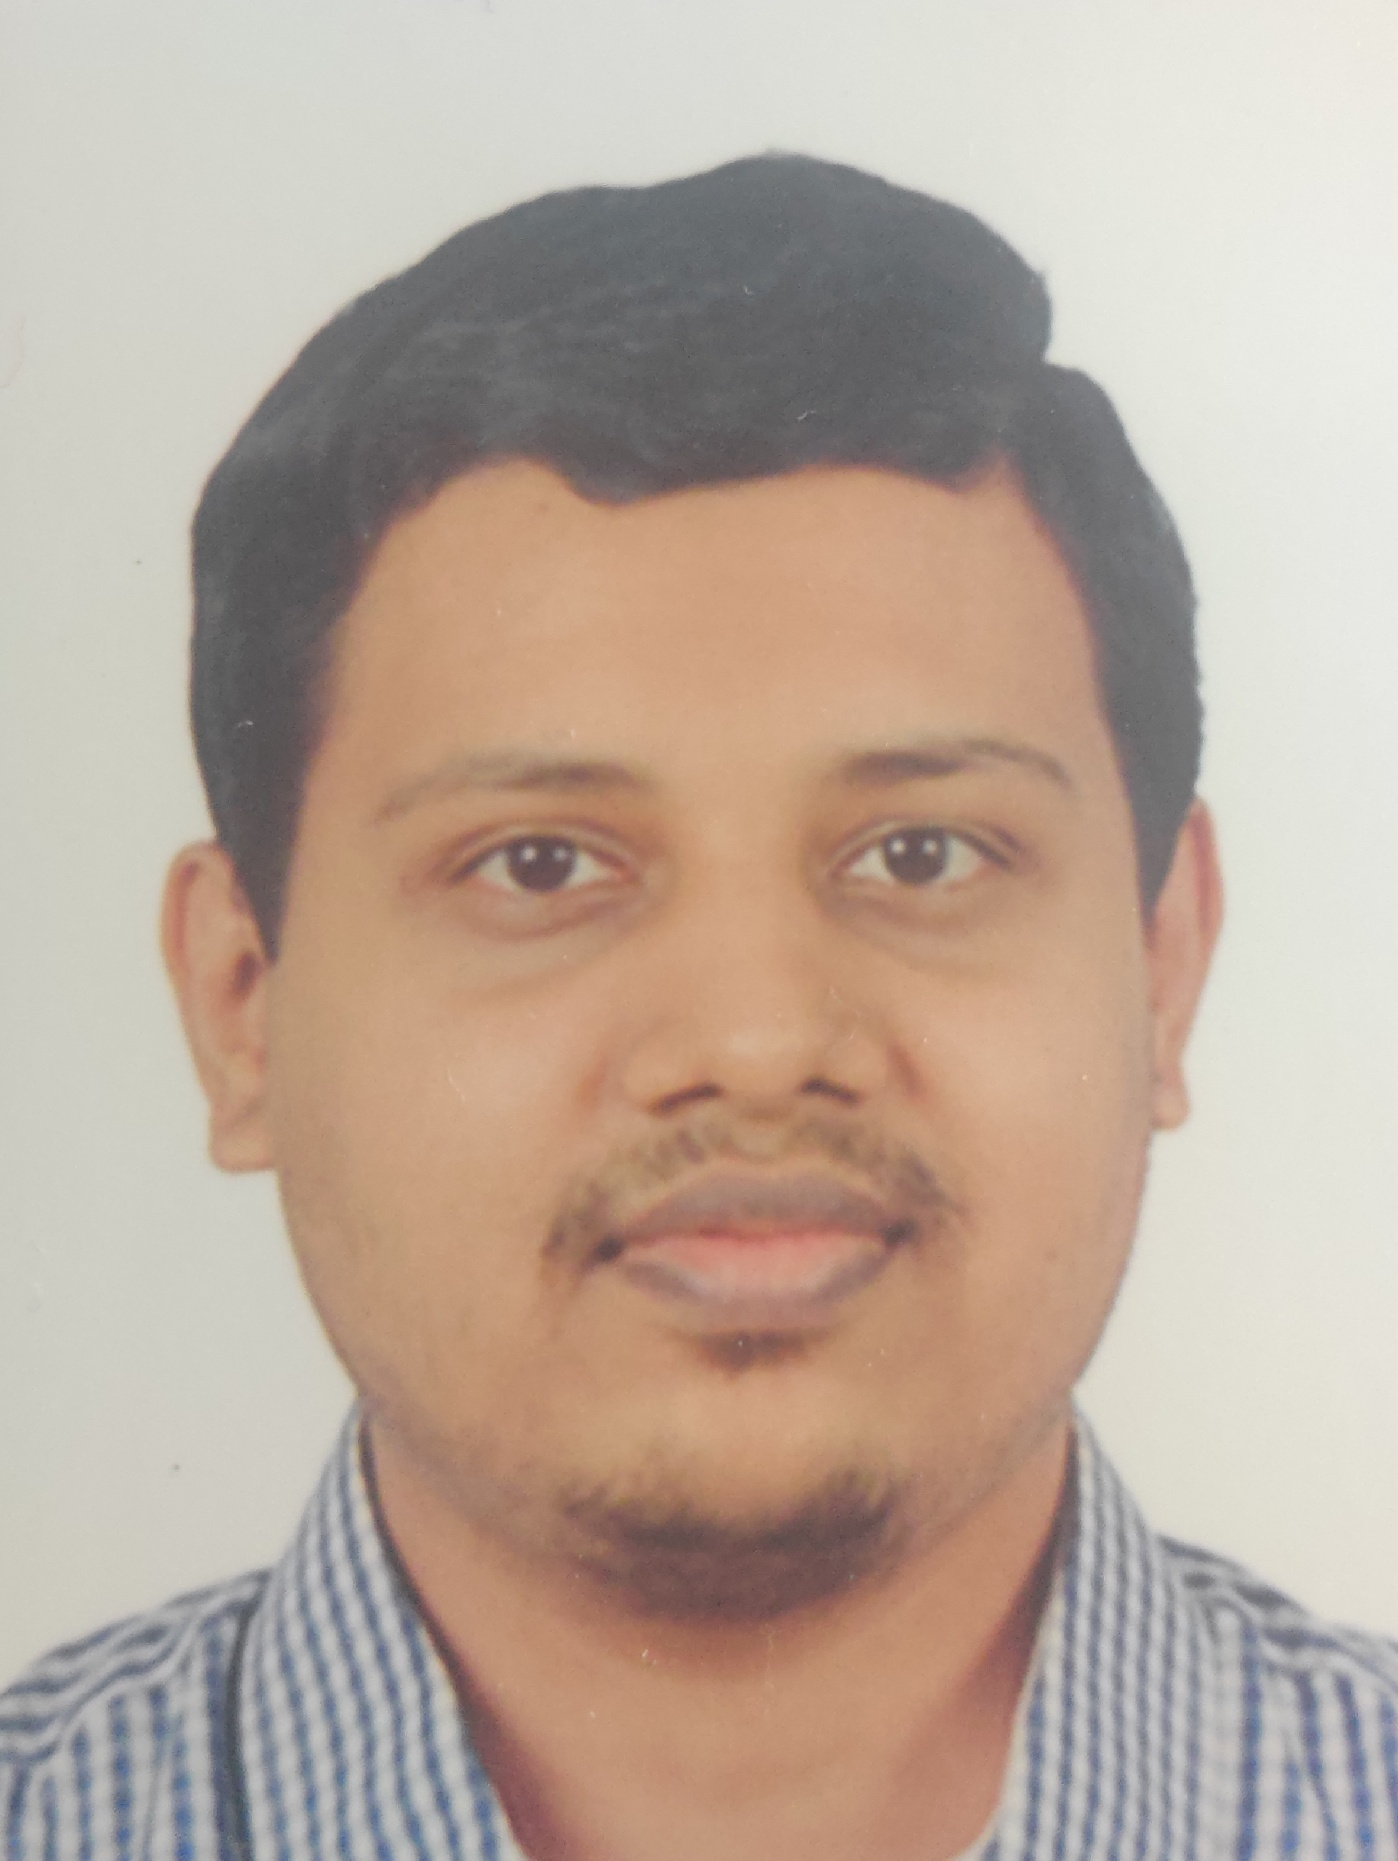
\includegraphics[width=1\linewidth]{images/abhishek_r_s.jpg}
    \end{wrapfigure}
    \paragraph{}
\end{comment}

%----------HEADING-----------------
\begin{tabular*}{\textwidth}{l@{\extracolsep{\fill}}r}
    \textbf{{\Large Abhishek Ramanathapura Satyanarayana}}
    \\
    {Groningen, the Netherlands}
    \\
    \href{mailto:abhishek.r.satyanarayana.4@gmail.com}{\faEnvelope} \hspace{0.1cm} \href{mailto:abhishekrsatyanarayana@gmail.com}{\faEnvelope} \hspace{0.1cm}
    \href{https://github.com/AbhishekRS4/}{\faGithub} \hspace{0.1cm} 
    \href{https://abhishekrs4.github.io/}{\faGithubSquare} \hspace{0.1cm} 
    \href{https://www.linkedin.com/in/abhishek-ramanathapura-satyanarayana-862608a0/}{\faLinkedinSquare} \hspace{0.1cm}
    \href{https://github.com/AbhishekRS4/cv_main/blob/master/cv_abhishek_r_s.pdf}{\faFilePdfO} \hspace{0.1cm}
    \href{https://drive.google.com/drive/folders/0Byk-dMy2pBxeX21IbmRlWFExNFk?usp=sharing}{\faFilesO}
    \\
    
\end{tabular*}

%-----------RESEARCH INTERESTS-----------------
\section{Research Interests}
    \resumeSubHeadingListStart
        \item{Artificial Intelligence, Machine Learning, Deep Learning, Computer Vision, Robot Perception}\\
    \resumeSubHeadingListEnd

%-----------EDUCATION-----------------
\section{Education}
    \resumeSubHeadingListStart
        \resumeSubheading
            {\underline{\href{https://www.rug.nl/masters/artificial-intelligence/}{University of Groningen [RUG]}}}{Groningen, The Netherlands}
            {M.Sc. in Artificial Intelligence}{Sep 2021 - present}

        \resumeSubheading
            {\underline{\href{https://www.rug.nl/education/honours-college/htsm-masterprogramme/}{Honours College, University of Groningen}}}{Groningen, The Netherlands}
            {Honours Master's in High Tech Systems and Materials (HTSM)}{Nov 2021 - Jun 2023}
        
        \resumeSubheading
            {\underline{\href{https://www.nitk.ac.in/}{National Institute of Technology Karnataka [NITK]}}}{Surathkal, Mangaluru,  India}
            {B.Tech. in Information Technology, CGPA: 8.3/10}{Jul 2012 - May 2016}
    \resumeSubHeadingListEnd

%-----------EXPERIENCE-----------------
\section{Experience}
    \resumeSubHeadingListStart
        \resumeSubheading{\underline{\href{https://www.rug.nl/fse/}{FSE, University of Groningen}}}{Groningen, The Netherlands}{Teaching Assistant (Part-time)}{May 2023 - Jun 2023}
            \resumeSubHeadingListStart
                \resumeItem{Teaching Assistant (TA)}{Part-time work as a TA for  \href{https://ocasys.rug.nl/current/catalog/course/WMAI019-05}{\textit{Handwriting Recognition}} course offered by Faculty of Science and Engineering (FSE), University of Groningen.}
            \resumeSubHeadingListEnd
        
        \resumeSubheading{\underline{\href{https://www.rug.nl/fse/}{FSE, University of Groningen}}}{Groningen, The Netherlands}{Teaching Assistant (Part-time)}{Feb 2023 - Apr 2023}
            \resumeSubHeadingListStart
                \resumeItem{Teaching Assistant (TA)}{Part-time work as a TA for  \href{https://ocasys.rug.nl/current/catalog/course/WMAI017-05}{\textit{Deep Learning}} and \href{https://ocasys.rug.nl/current/catalog/course/WMCS015-05}{\textit{Computer Vision}} courses offered by Faculty of Science and Engineering (FSE), University of Groningen.}
            \resumeSubHeadingListEnd
    
        \resumeSubheading{\underline{\href{https://www.rug.nl/fse/}{FSE, University of Groningen}}}{Groningen, The Netherlands}{Teaching Assistant (Part-time)}{Sep 2022 - Nov 2022}
            \resumeSubHeadingListStart
                \resumeItem{Teaching Assistant (TA)}{Part-time work as a TA for  \href{https://www.rug.nl/ocasys/fwn/vak/show?code=WMAI003-05}{\textit{Cognitive Robotics}} and \href{https://www.rug.nl/ocasys/fwn/vak/show?code=WMCS002-05}{\textit{Introduction to Data Science}} courses offered by Faculty of Science and Engineering (FSE), University of Groningen.}
            \resumeSubHeadingListEnd    
    
        \resumeSubheading{\underline{Tata Steel in Europe}}{IJmuiden, The Netherlands}{Summer AI Intern}{Jul 2022 - Aug 2022}
            \resumeSubHeadingListStart
                \resumeItem{Dutch Summer of AI}{This summer internship was a part of the \href{https://www.summerof.ai/}{Dutch Summer of AI}, edition 2022. Our team won the award for Solving the Most Valuable Problem.}
                \resumeItem{Internship work}{Worked on supervised and unsupervised deep learning methods to classify and cluster images with steel surface defects.}
            \resumeSubHeadingListEnd

        \resumeSubheading{\underline{\href{https://www.umcg.nl/}{UMCG}}}{Groningen, The Netherlands}{Teaching Assistant (Part-time)}{Jun 2022 - Jul 2022}
            \resumeSubHeadingListStart
                \resumeItem{\href{https://www.rug.nl/research/gradschool-medical-sciences/summer-schools/data-science-and-ai/}{Summer School Data Science and AI in Health}}{Part-time work as a Teaching Assistant during the Summer School, edition 2022.}
            \resumeSubHeadingListEnd

        \resumeSubheading{\underline{{Philips Consumer Lifestyle B.V.}}}{Drachten, The Netherlands}{Internship (Part-time)}{Nov 2021 - Jul 2022}
            \resumeSubHeadingListStart
                \resumeItem{{Industrial Challenge Internship}}{Part-time internship work as a part of HTSM Honours Master's.}
            \resumeSubHeadingListEnd

        \resumeSubheading{\underline{\href{https://www.atimotors.com/}{Ati Motors}}}{Bengaluru, India}{Research Associate (Machine Learning) in Autonomy}{Sep 2017 - Jun 2021}
            \resumeSubHeadingListStart
                \resumeItem{Machine learning}
                {Worked on research, prototype, development, and deployment of Machine Learning, Deep Learning, Computer Vision, Robot Perception, and Algorithm solutions for autonomous cargo vehicles. This involved using the LiDAR and multi-modal camera data (i.e. RGBD) for developing various ML pipelines with a focus on object classification in 2D images, object detection in 2D images, semantic segmentation in 2D images, and semantic segmentation in 3D LiDAR point cloud data.}
                \resumeItem{HW benchmarking}{Benchmarking of various ML models that were developed on multiple HW devices such as Nvidia's server GPUs, Intel Movidius stick, and Nvidia Xavier embedded development board.}
                \resumeItem{Sensor drivers}{Active involvement in prototype, development, deployment, and testing of various LiDAR and camera sensor drivers (including multi-modal i.e. RGBD camera).}
                \resumeItem{Sensor data pipelines}{Active involvement in development, deployment, and testing of various raw and derived sensor data pipelines.}
                \resumeItem{Testing}{Active involvement in testing various algorithm pipelines on prototype and production vehicles.}
                \resumeItem{Demos and deployment}{Active involvement in multiple potential customer demos and successful customer deployment activities at customer sites. This includes Ati's successful first and further customer deployments.}
            \resumeSubHeadingListEnd

        \resumeSubheading{\underline{\href{https://iisc.ac.in/}{Indian Institute of Science}}}{Bengaluru, India}{Project Assistant Intern at HPC Lab in SERC}{Jun 2016 - Dec 2016}
            \resumeSubHeadingListStart
                \resumeItem{Professor guide}{Prof. R Govindarajan}
                \resumeItem{Parallel programming}{Worked on implementation and benchmarking of data parallel algorithms to achieve high performance on hardware accelerators using APIs - CUDA C, OpenCL, OpenMP.}
            \resumeSubHeadingListEnd
        \resumeSubheading{\underline{\href{https://careers.jpmorgan.com/us/en/about-us/locations/mumbai}{J P Morgan Chase}}}{Mumbai, India}{Technology Analyst Intern in Investment Banking}{May 2015 - Jul 2015}
            \resumeSubHeadingListStart
                \resumeItem{Data analysis}{Worked on data analysis of real-time transaction data.}
            \resumeSubHeadingListEnd
    \resumeSubHeadingListEnd

\begin{comment}
%-----------PROFILES-----------------
\section{Profiles}
    \resumeSubHeadingListStart
        \item{Linkedin: }
        \item{Github: \href{https://github.com/AbhishekRS4/}{\faGithub}}
            \item{Kaggle: \underline{\href{https://www.kaggle.com/abhishekrs4/}{https://www.kaggle.com/abhishekrs4/}}}
        
        
    \resumeSubHeadingListEnd
\end{comment}

%-----------PROJECTS-----------------
\begin{comment}
\section{Projects}
    \resumeSubHeadingListStart
        \resumeSubItem{Developed a visualizer dashboard for analysis of data of Covid-19 infection in India}
        {This tool relies on data collected by an open-source project \href{https://www.covid19india.org/}{https://www.covid19india.org/}. The visualizer dashboard has multiple options to visualize Covid-19 infection data in India.}
        \resumeSubItem{Implementation of various Convolutional Neural Network models for Semantic Segmentation on Cityscapes and CamVid datasets}
        {Implemented various CNN models such as FCN, SegNet, UNet, LinkNet, PSPNet, DeepLab\_v3, Tiramisu on custom classes. The experiment is to study the various ideas proposed in research papers and its effects on performance of the model on validation set.}
        \resumeSubItem{Participated in TGS Salt Identification Challenge hosted on Kaggle}
        {Implemented custom CNN model using ideas from various research papers for salt segmentation in Kaggle competition. The model scored 0.811743 IoU on private test set. Our team finished in top 53\% of the leaderboard.}
        \resumeSubItem{Implementation of Convolutional Neural Network model based on Nvidia's research paper End to End Learning for Self-Driving Cars}
        {Implemented CNN model to predict steering angle from image on California Highway road dataset. The experiment is to reproduce the findings of the research paper that a CNN model can learn to predict steering angle from an image with reasonable performance.}
        \resumeSubItem{Classification of traffic sign images using German Traffic Sign Recognition Benchmark dataset}
        {Implemented CNN model for classification of traffic sign images on GTSRB dataset with 43 classes. The model scored 97.7\% accuracy on test set.}
        \resumeSubItem{Boston House Price Prediction}
        {Supervised Learning task of predicting the house median value for the Boston House dataset using various Regression techniques, Artificial Neural Network as part of mini project for Soft Computing Course. Tuning the hyper-parameters of ANN scored the best rmse among the various models.}
        \resumeSubItem{Comparison of Artificial Neural Network, Support Vector Regression (SVR), Genetic Algorithm-SVR}
        {Studied and experimented an IEEE paper which compares the three models ANN, SVR and GA-SVR using open source R and its packages as part of mini project for Data Warehousing and Data Mining Course. Tuning the hyper-parameters of ANN proved to be the best among the three models.}
        \resumeSubItem{Classification of handwritten digit images using MNIST dataset}
        {Implemented CNN model for classification of handwritten digit images on MNIST dataset with 10 classes. The model scored 99.47\% accuracy on test set.}
        \resumeSubItem{Denial of Service attack identification based on Reputation based Trust in Wireless Sensor Networks}
        {Identification of DoS attack based on Reputation based Trust in WSN using three different models RFSN model (a mathematical approach), human behavior model and ant colony optimization algorithm. This research was my Major Project (final year). We demonstrated that RFSN model could outperform other models in identification of the DoS attack.}
        \resumeSubItem{Data Parallel Algorithms}
        {Implementation of various Data Parallel Algorithms in OpenMP and CUDA C as part of Parallel Computing Course.}
        \resumeSubItem{Implementation of Machine Learning Algorithms}
        {Implemented various Machine learning algorithms in Python.}
    \resumeSubHeadingListEnd
\end{comment}

% --------PROGRAMMING SKILLS------------
\section{Programming languages and Tech skills}
    \resumeSubHeadingListStart
        \resumeSubItem{Programming languages}
        {Python, C, C++, Java, Matlab}
        \resumeSubItem{Database}
        {SQLite, MySQL}
        \resumeSubItem{Version control}
        {Git}
        %\resumeSubItem{Open Source tools}
        % {numpy, scipy, pandas, matplotlib, scikit-learn, opencv, tensorflow, % pytorch, cupy, streamlit}
    \resumeSubHeadingListEnd

% --------ONLINE COURSES------------
\section{Self Learning Courses}
    \resumeSubHeadingListStart
        \item{Machine Learning, Coursera (Certification)}\\
        \item{Mathematics for Machine Learning Specialization, Coursera (Certification)}\\
        \item{Deep Learning Specialization, Coursera (Certification)}\\
        \item{Applied Data Science Specialization, Coursera (Certification)}\\
        \item{Python for Everybody Specialization, Coursera (Certification)}\\
        \item{Robotics - Perception, Coursera (Certification)}\\
        \item{An Intuitive Introduction to Probability, Coursera (Certification)}\\
        \item{Data Science Math Skills, Coursera (Certification)}\\
        \item{Fibonacci Numbers and Golden Ration, Coursera (Certification)}\\
        \item{Parallel Programming and Optimization for Intel Architectures, Colfax Research (Certification)}\\
    \resumeSubHeadingListEnd

% --------AWARDS------------
\section{Notable Awards and Achievements}
    \resumeSubHeadingListStart
        \resumeSubheading{Dutch Summer of AI, edition 2022}{Amsterdam, The Netherlands}{}{2021-2022}
        \resumeSubHeadingListStart
            \resumeItem{Summer AI Intern at Tata Steel in Europe}{Our team won the award for Solving the Most Valuable Problem, among 9 participating teams at the Dutch Summer of AI, edition 2022.}
        \resumeSubHeadingListEnd
    
        \resumeSubheading{Beta Business Days, edition 2022}{Groningen, The Netherlands}{}{2021-2022}
        \resumeSubHeadingListStart
            \resumeItem{B \& S case study - Text recognition challenge}{Won the best solution award by developing a web application solution using the cognitive services API offered by Azure.}
        \resumeSubHeadingListEnd
        
        \resumeSubheading{Acute Myeloid Leukemia Prediction Challenge}{Groningen, The Netherlands}{}{2021-2022}
        \resumeSubHeadingListStart
            \resumeItem{Acute Myeloid Leukemia Prediction Challenge}{Our team won the $2^{nd}$ best performer award in the Acute Myeloid Leukemia Prediction Challenge conducted as part of the Introduction to Data Science Master's course at the University of Groningen}
        \resumeSubHeadingListEnd
    \resumeSubHeadingListEnd

% --------AWARDS------------ [old]
\begin{comment}
    \resumeSubheading{All India Engineering Entrance Examination [now replaced by JEE mains]}{India}{Secured a national rank of 6279 among 1200000 candidates}{2011-2012}
    \resumeSubheading{Karnataka Common Entrance Test [KCET] for Engineering}{India}{Secured a state rank of 404 among 80000 candidates}{2011-2012}
    \resumeSubheading{Pre-university Science quiz}{India}{3\textsuperscript{rd} prize in science quiz}{2011-2012}
    \resumeSubheading{Annual high school awards}{India}{3\textsuperscript{rd} best outgoing student award}{2009-2010}
    \resumeSubheading{Bharath ko jano (translation: Know about India)}{India}{2\textsuperscript{nd} prize in inter-high school quiz competition conducted by Bharath Vikas Parishad}{2009-2010}
    \resumeSubheading{Annual high school quiz competition}{India}{2\textsuperscript{nd} prize}{2009-2010}
    \resumeSubheading{Annual high school quiz competition}{India}{1\textsuperscript{st} prize}{2008-2009}
    \resumeSubheading{National Science Olympiad}{India}{1\textsuperscript{st} prize for my high school}{2007-2008}
    \resumeSubheading{Chess competitions in School}{India}{Various prizes in primary and high school including 3 first and 2 runner-up prizes}{2005-2010}
    \resumeSubheading{All India General Knowledge by Center for Human Resource Development}{India}{Completion of CHRD general knowledge competition with distinction}{2005-2006}
\end{comment}

% --------EXTRA CURRICULAR ACTIVITY------------
\section{Extra Curricular Activities}
    \resumeSubHeadingListStart
        \resumeSubheading{\underline{\href{https://www.imtex.in/}{IMTEX FORMING}} 2020 held at BIEC}{Bengaluru, India}{Represented Ati Motors}{Jan 2020}
        
        \resumeSubheading{Poster session held at Indian Institute of Science}{Bengaluru, India}{Represented Ati Motors}{Jul 2019}
        
        \resumeSubheading{\underline{\href{https://incident.nitk.ac.in/}{Incident-16}} (cultural festival of NITK)}{Surathkal, Mangaluru, India}{Team member that conducted the Gaming events of Incident-16}{Mar 2016}
        
        \resumeSubheading{TECHeshi’s castle at NITK IEEE tech festival}{Surathkal, Mangaluru, India}{Team member that conducted the event}{Dec 2012 - Jan 2013}
        
        %\resumeSubheading{Bengaluru district level science exhibition}{Bengaluru, India}{Presented on water conservation using rain water harvesting}{2007-2008}
        
        %\resumeSubheading{\underline{\href{https://www.janaagraha.org/bala-janaagraha/}{Bala Janagraha Civic learning programme}}}{Bengaluru, India}{Completed the civic learning programme in high school}{2007-2008}
    \resumeSubHeadingListEnd

% --------References------------
\section{References}
    \resumeSubHeadingListStart
        \item
        {Dr. Geetha V \\
        Assistant Professor \\
        Department of Information Technology \\
        National Institute of Technology Karnataka, India \\
        Email: \underline{\href{mailto:geethav@nitk.edu.in}{geethav@nitk.edu.in}} \\
        Website: \underline{\href{https://infotech.nitk.ac.in/faculty/geetha-v}{https://infotech.nitk.ac.in/faculty/geetha-v}}}
        \item
        {Dr. Jaidhar C D \\
        Associate Professor \\
        Department of Information Technology \\
        National Institute of Technology Karnataka, India \\
        Email: \underline{\href{mailto:jaidharcd@nitk.edu.in}{jaidharcd@nitk.edu.in}} \\
        Website: \underline{\href{https://infotech.nitk.ac.in/faculty/jaidhar-c-d}{https://infotech.nitk.ac.in/faculty/jaidhar-c-d}}}
    \resumeSubHeadingListEnd

%-------------------------------------------
\end{document}
